\documentclass[11pt,a4paper]{article}

% ----- PACKAGES -----
\usepackage[utf8]{inputenc}
\usepackage[T1]{fontenc}
\usepackage{mathpazo}
\usepackage{amsmath,amssymb,amsfonts,bm}
\usepackage{geometry}
\usepackage{xcolor}
\usepackage{booktabs}
\usepackage{colortbl}
\usepackage{multirow}
\usepackage[many]{tcolorbox}
\usepackage{titlesec}
\usepackage{microtype}
\usepackage{hyperref}
\usepackage{graphicx}
\usepackage{tikz}
\usepackage{caption}
\usepackage{subcaption}
\usetikzlibrary{calc,arrows.meta,decorations.pathreplacing,decorations.markings,positioning}

% ----- GEOMETRY & COLORS -----
\geometry{top=1.2in, bottom=1.2in, left=1in, right=1in}

\definecolor{TitleBlue}{RGB}{26, 61, 109}
\definecolor{Cat1Red}{RGB}{186, 57, 57}
\definecolor{Cat2green}{RGB}{32, 120, 115}
\definecolor{Cat3Purple}{RGB}{110, 48, 114}
\definecolor{MathBg}{RGB}{245, 247, 250}
\definecolor{IntuitionGold}{RGB}{184, 134, 11}
\definecolor{IntuitionBg}{RGB}{253, 248, 233}
\definecolor{LabGreen}{RGB}{44, 110, 73}
\definecolor{LabBg}{RGB}{238, 246, 240}

\definecolor{RodOrange}{RGB}{248, 138, 53}
\definecolor{SampleYellow}{RGB}{231, 198, 73}
\definecolor{ArmBlue}{RGB}{86, 161, 232}
\definecolor{Armgreen}{RGB}{52, 196, 165}
\definecolor{TargetGreen}{RGB}{103, 198, 102}

\hypersetup{
    colorlinks=true,
    linkcolor=TitleBlue,
    urlcolor=TitleBlue
}

\titleformat{\section}{\Large\bfseries\color{TitleBlue}}{\thesection}{1em}{}[{\color{TitleBlue}\titlerule}]
\titleformat{\subsection}{\large\bfseries\color{TitleBlue}}{\thesubsection}{1em}{}

\captionsetup{font=small, labelfont={bf,color=TitleBlue}, textfont=it}

\tcbset{
    masterbox/.style={
        enhanced, breakable,
        fonttitle=\bfseries\large, coltitle=white,
        attach boxed title to top left={yshift=-2mm, xshift=5mm},
        boxed title style={sharp corners},
        boxrule=1pt, arc=3mm,
        top=15pt, bottom=10pt, left=10pt, right=10pt
    },
    mathbox/.style={
        enhanced,
        colback=MathBg, colframe=TitleBlue!40,
        boxrule=0.5pt, arc=2mm, drop fuzzy shadow
    },
    notebox/.style={
        enhanced,
        colback=TitleBlue!4, colframe=TitleBlue!50,
        boxrule=0.5pt, arc=1.5mm,
        left=8pt, right=8pt, top=6pt, bottom=6pt
    }
}

\newtcolorbox{intuition}[1][\unskip]{
    enhanced, breakable,
    colback=IntuitionBg, colframe=IntuitionGold,
    boxrule=0.6pt, arc=1.5mm,
    left=10pt, right=10pt, top=6pt, bottom=8pt,
    title={\textcolor{white}{\textsf{Intuition} \;\textbar\; #1}},
    fonttitle=\small\bfseries, coltitle=white,
    boxed title style={colback=IntuitionGold, sharp corners},
    attach boxed title to top left={yshift=-2mm, xshift=8pt}
}

\newtcolorbox{labexercise}[1][\unskip]{
    enhanced, breakable,
    colback=LabBg, colframe=LabGreen,
    boxrule=0.7pt, arc=1.5mm,
    left=10pt, right=10pt, top=6pt, bottom=8pt,
    title={\textcolor{white}{\textsf{Lab exercise} \;\textbar\; #1}},
    fonttitle=\small\bfseries, coltitle=white,
    boxed title style={colback=LabGreen, sharp corners},
    attach boxed title to top left={yshift=-2mm, xshift=8pt}
}

\newtcolorbox{physbox}[1][]{
    masterbox,
    title=Category 1 \;\textbar\; Controllability singularities,
    colback=Cat1Red!5, colframe=Cat1Red,
    boxed title style={colback=Cat1Red}, #1
}
\newtcolorbox{obsbox}[1][]{
    masterbox,
    title=Category 2 \;\textbar\; Observability singularities,
    colback=Cat2green!5, colframe=Cat2green,
    boxed title style={colback=Cat2green}, #1
}
\newtcolorbox{dynbox}[1][]{
    masterbox,
    title=Category 3 \;\textbar\; Mechanical instabilities,
    colback=Cat3Purple!5, colframe=Cat3Purple,
    boxed title style={colback=Cat3Purple}, #1
}

\title{\vspace{-2em}\textbf{\Huge An Introduction to\\[0.15em] Jacobian-Based Shape Servoing}\\[0.6em]
\Large \color{gray} Data-driven estimation and control for
model-free deformable-object manipulation}
\author{Lecture notes by Ignacio Cuiral-Zueco, with accompanying Python lab session}
\date{}

\begin{document}

\maketitle

\begin{abstract}
\noindent \emph{Shape servoing} is the task of bringing a deformable object to a desired
target shape by means of robot manipulation. When no mechanical model of the object is
available, the control law is organised around an \emph{interaction Jacobian}: the local
linear map relating gripper motion to the change it produces in the object's shape, as
measured by a visual sensor such as an RGB-D camera. This Jacobian can be estimated directly
from data and then inverted to define the shape controller. These notes develop the method
through a single running example, a planar setup in which two 2D robots act on an elastic rod.
We define the actuation and shape feature spaces, examine how the object's shape can be
represented in several ways, explain how the Jacobian is estimated, and show how its
pseudo-inverse closes the control loop. We then analyse the three characteristic ways in which
a Jacobian-based shape control loop fails: loss of controllability, loss of observability, and
mechanical instability. Each mathematical concept is accompanied by a short ``intuition'' box,
and each section closes with a Python exercise from the accompanying lab session, so that a
complete data-driven shape-servoing framework is built up incrementally.
\end{abstract}

\vspace{1em}
\tableofcontents
\vspace{1.5em}

% \begin{tcolorbox}[notebox]
% \textbf{Notation at a glance.}
% $\mathbf{x}$ is the rod's \emph{true physical state}, the equilibrium configuration it settles
% into; it is the output of the plant and is not measured directly.
% $\mathbf{s}\in\mathbb{R}^{n}$ is the \emph{feature} vector that a perception step extracts from $\mathbf{x}$
% ($n=2P=10$, from $P=5$ sampled points), the finite state the controller works with.
% $\mathbf{r}\in\mathbb{R}^{m}$ is the \emph{actuation} vector we command ($m=6$), the end-effector
% (EE) pose of the two grippers.
% $\mathbf{s}^{*}$ is the target and $\mathbf{e}=\mathbf{s}^{*}-\mathbf{s}$ the shape error.
% $\mathbf{J}\in\mathbb{R}^{n\times m}$ is the \emph{true} interaction Jacobian ($\dot{\mathbf{s}} = \mathbf{J}\dot{\mathbf{r}}$,
% set by the object's mechanics and unknown to the controller), and $\hat{\mathbf{J}}$ is its estimate.
% $\mathbf{J}^{+}$ denotes the Moore--Penrose pseudo-inverse.
% \end{tcolorbox}

% ===========================================================
\section{Setup}
\label{sec:setup}

Two planar arms hold an elastic rod by its endpoints. Each gripper has three independent
degrees of freedom (DoF): two translation DoFs and one orientation DoF. The current robot configuration can be 
represented through its end-effector (EE) pose vector
\[
    \mathbf{r} \;=\; [\,x_L,\, y_L,\, \theta_L,\;\; x_R,\, y_R,\, \theta_R\,]^{\top} \;\in\; \mathbb{R}^{m},
    \qquad m = 6,
\]
where the subscripts $L$ and $R$ denote the left and right grippers, $(x,y)$ is the gripper
position in the world frame, and $\theta$ denotes the EE orientation (its rotation axis is
perpendicular to the plane in which the setup is defined).

The rod is assumed to behave quasistatically, which means its physical state $\mathbf{x}$, a
continuous curve with infinitely many degrees of freedom, evolves only when the robots actuate
the rod through \textit{small} changes in their configuration $\mathbf{r}$. The continuous state
$\mathbf{x}$ cannot be measured directly from visual sensors, so shape servoing works instead with a
reduced representation of $\mathbf{x}$: a finite feature vector $\mathbf{s}\in\mathbb{R}^{n}$. In our 2D rod
example, the controller's actuation space is the six-dimensional end-effector pose vector
$\mathbf{r}$, and the feature space is the ten-dimensional vector $\mathbf{s}$ of sampled rod coordinates. We
sample $P=5$ points
along the rod (yellow dots in Figure~\ref{fig:setup}) and stack the planar coordinates
$(x_i,y_i)$ of the $i$-th sampled point into the feature vector
\[
    s \;=\; [\,x_1, y_1,\; x_2, y_2,\; \dots,\; x_P, y_P\,]^{\top} \;\in\; \mathbb{R}^{n},
    \qquad n = 2P = 10 \ \ (P=5).
\]
The control problem is to find the changes in EE pose $\mathbf{r}$ (i.e., the sequence of $\Delta\mathbf{r}$) that bring $\mathbf{s}$ as close as possible to the target value $\mathbf{s}^{*}$ that encodes the target shape.

\begin{tcolorbox}[notebox]
\textbf{One choice among many.} The pair $(\mathbf{r},\,\mathbf{s})$ used here is one simple example of an
\emph{actuation space} and a \emph{feature space}. Other definitions are possible: a 3D
actuation with three translation and three rotation DoF, or a feature vector $\mathbf{s}$ built
from edge vectors, curvatures, contour descriptors, or visual feature descriptors rather
than 2D point coordinates. We adopt the pair above for clarity;
\S\ref{sec:representation} discusses alternative choices of $\mathbf{s}$ and their properties.
\end{tcolorbox}

\begin{figure}[h!]
    \centering
    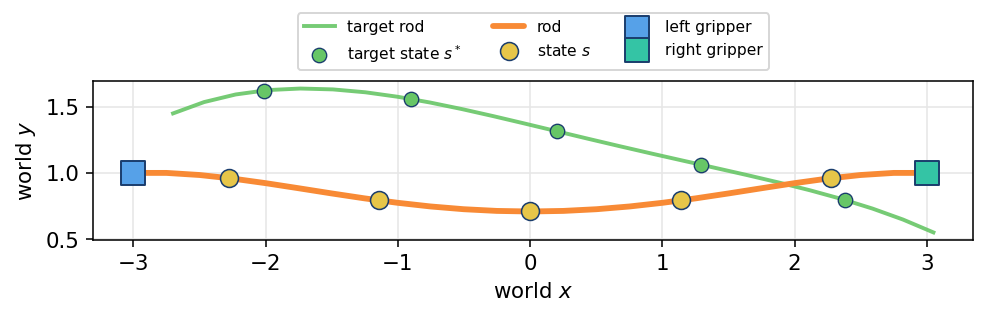
\includegraphics[width=0.82\linewidth]{figs/fig_setup.png}
    \caption{The control problem. Two grippers (blue, green squares) clamp an elastic
    rod (orange). Five points sampled along the rod (yellow) form the measured feature state
    $\mathbf{s}$. The target shape (green) and its sampled state $\mathbf{s}^{*}$ define where we want the
    rod to be; the task is to bring $\mathbf{s}$ to $\mathbf{s}^{*}$ by means of gripper actions.}
    \label{fig:setup}
\end{figure}

\noindent We assume no knowledge of the physical model of the rod: no bending stiffness, no mass,
and no boundary conditions. Everything the model-free controller needs is the local
response of the measured features $\mathbf{s}$ (geometric data) with respect to changes in the robot configuration $\mathbf{r}$.

The shape servoing system runs in two phases, shown in Figures~\ref{fig:offline} and~\ref{fig:online}.
In the \emph{offline} phase, before any control takes place, the robots execute an exploration
sequence (small end-effector moves applied one degree of freedom at a time), and the
measured responses are fit by least squares into an initial Jacobian estimate
$\hat{\mathbf{J}}^{(0)}$. In the \emph{online} phase, the controller compares the measured features
$\mathbf{s}$ with the target $\mathbf{s}^{*}$, and turns the feature error $\mathbf{e}$ into robot actions $\Delta\mathbf{r}$ through the
inverse (pseudoinverse) of the Jacobian matrix. Such actions produce a new rod state $\mathbf{x}$, and the perception block maps $\mathbf{x}$ to the new
features $\mathbf{s}$. A Broyden estimator (to be introduced) refines $\hat{\mathbf{J}}$ online using the action values
$\Delta\mathbf{r}$ and their resulting feature response $\Delta\mathbf{s}$. Each block is detailed in the following sections:
\S\ref{sec:representation} feature extraction, \S\ref{sec:jacobian} offline Jacobian estimation and its conditioning,
and \S\ref{sec:estimation} closing the loop and the online Broyden update.

\begin{figure}[h!]
\centering
\resizebox{\linewidth}{!}{%
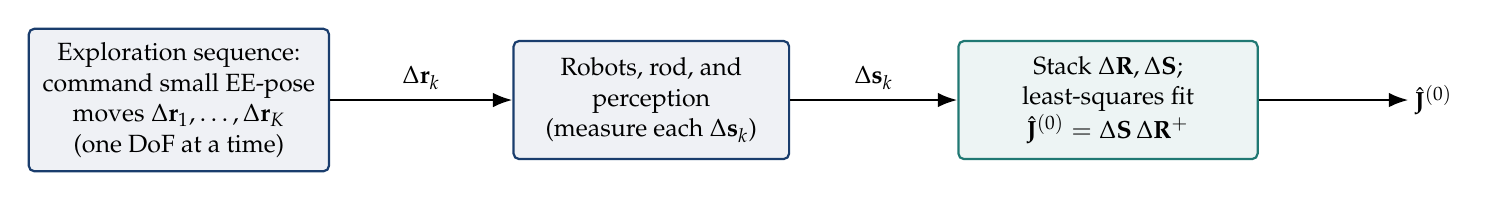
\begin{tikzpicture}[>=Latex, font=\small,
  blk/.style={draw=TitleBlue, line width=0.8pt, rounded corners=2pt, fill=TitleBlue!7,
              align=center, inner sep=5pt, minimum height=1.5cm, minimum width=3.5cm},
  fit/.style={draw=Cat2green, line width=0.8pt, rounded corners=2pt, fill=Cat2green!8,
              align=center, inner sep=5pt, minimum height=1.5cm, minimum width=3.8cm},
  sig/.style={->, line width=0.9pt}]
  \node[blk] (cal) at (0,0)    {Exploration sequence:\\command small EE-pose\\moves $\Delta\mathbf{r}_1,\dots,\Delta\mathbf{r}_K$\\(one DoF at a time)};
  \node[blk] (sys) at (6.0,0)  {Robots, rod, and\\perception\\(measure each $\Delta\mathbf{s}_k$)};
  \node[fit] (fit) at (11.8,0) {Stack $\Delta\mathbf{R},\Delta\mathbf{S}$;\\least-squares fit\\$\hat{\mathbf{J}}^{(0)}=\Delta\mathbf{S}\,\Delta\mathbf{R}^{+}$};
  \draw[sig] (cal) -- node[above]{$\Delta\mathbf{r}_k$} (sys);
  \draw[sig] (sys) -- node[above]{$\Delta\mathbf{s}_k$} (fit);
  \draw[sig] (fit.east) -- ++(1.9,0) node[right, inner sep=2pt]{$\hat{\mathbf{J}}^{(0)}$};
\end{tikzpicture}}
\caption{\textbf{Offline initialisation.} The robots run an exploration sequence, moving
one end-effector degree of freedom at a time; each commanded $\Delta\mathbf{r}_k$ and its
measured feature response $\Delta\mathbf{s}_k$ are stacked into matrices $\Delta\mathbf{R},\Delta\mathbf{S}$ and fit by
least squares to obtain the initial Jacobian estimate $\hat{\mathbf{J}}^{(0)}$, which is later used on the online control loop.}
\label{fig:offline}
\end{figure}

\begin{figure}[h!]
\centering
\resizebox{\linewidth}{!}{%
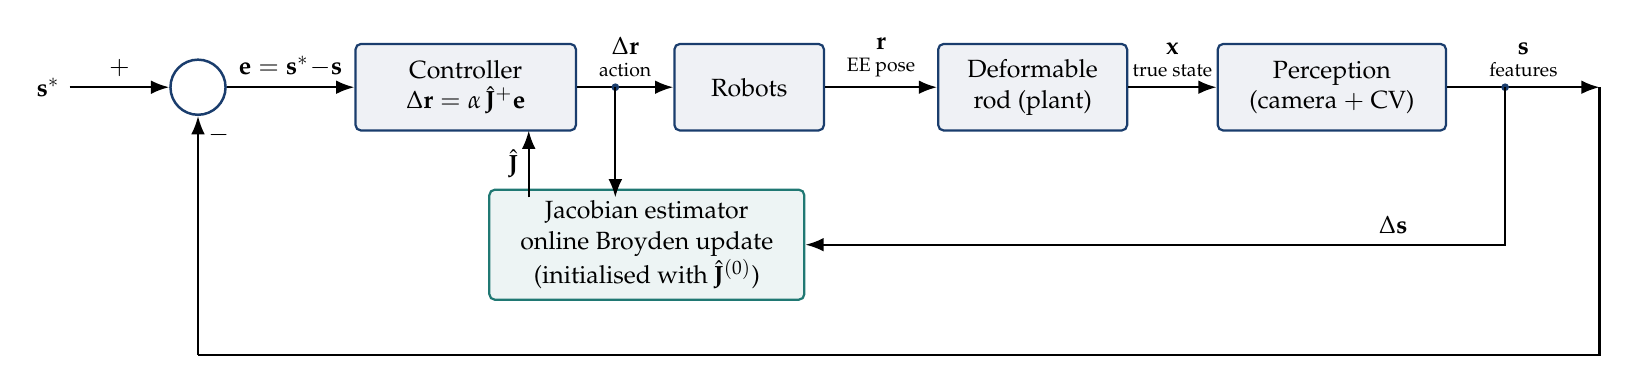
\begin{tikzpicture}[>=Latex, font=\small,
  blk/.style={draw=TitleBlue, line width=0.8pt, rounded corners=2pt, fill=TitleBlue!7,
              align=center, inner sep=4pt, minimum height=1.1cm},
  est/.style={draw=Cat2green, line width=0.8pt, rounded corners=2pt, fill=Cat2green!8,
              align=center, inner sep=4pt, minimum height=1.2cm, minimum width=4.0cm},
  sum/.style={draw=TitleBlue, line width=0.9pt, circle, minimum size=7mm, inner sep=0pt},
  sig/.style={->, line width=0.8pt},
  lab/.style={above, align=center, font=\small}]

  % --- forward path ---
  \node[sum] (sum) at (0,0) {};
  \node[blk, minimum width=2.8cm] (ctrl) at (3.4,0)  {Controller\\$\Delta\mathbf{r}=\alpha\,\hat{\mathbf{J}}^{+}\mathbf{e}$};
  \node[blk, minimum width=1.9cm] (rob)  at (7.0,0)  {Robots};
  \node[blk, minimum width=2.4cm] (rod)  at (10.6,0) {Deformable\\rod (plant)};
  \node[blk, minimum width=2.9cm] (perc) at (14.4,0) {Perception\\(camera $+$ CV)};

  \node (ref) at (-1.9,0) {$\mathbf{s}^{*}$};
  \draw[sig] (ref)  -- node[pos=0.5, above, font=\small]{$+$} (sum);
  \draw[sig] (sum)  -- node[lab]{$\mathbf{e}=\mathbf{s}^{*}\!-\!\mathbf{s}$} (ctrl);
  \draw[sig] (ctrl) -- node[lab]{$\Delta\mathbf{r}$\\[-3pt]{\scriptsize action}} (rob);
  \draw[sig] (rob)  -- node[lab]{$\mathbf{r}$\\[-3pt]{\scriptsize EE pose}} (rod);
  \draw[sig] (rod)  -- node[lab]{$\mathbf{x}$\\[-3pt]{\scriptsize true state}} (perc);
  \coordinate (sout) at (17.8,0);
  \draw[sig] (perc) -- node[lab]{$\mathbf{s}$\\[-3pt]{\scriptsize features}} (sout);

  % --- negative feedback along the bottom ---
  \draw[line width=0.8pt] (sout) -- (17.8,-3.4) -- (0,-3.4);
  \draw[sig] (0,-3.4) -- node[pos=0.92, right, font=\small]{$-$} (sum);

  % --- online Jacobian estimator ---
  \node[est] (est) at (5.7,-2.0) {Jacobian estimator\\online Broyden update\\(initialised with $\hat{\mathbf{J}}^{(0)}$)};
  \fill[TitleBlue] (5.3,0) circle (1.4pt);
  \fill[TitleBlue] (16.6,0) circle (1.4pt);
  \draw[sig] (4.2,-1.4) -- node[left, pos=0.5, font=\small]{$\hat{\mathbf{J}}$} (4.2,-0.55);
  \draw[sig] (5.3,0) -- (5.3,-1.4);
  \draw[sig] (16.6,0) -- (16.6,-2.0) -- node[above, pos=0.16, font=\small]{$\Delta\mathbf{s}$} (est.east);
\end{tikzpicture}}
\caption{\textbf{Online control loop.} The forward path (blue) turns the shape error
$\mathbf{e}=\mathbf{s}^{*}-\mathbf{s}$ into robot actions $\Delta\mathbf{r}$; the rod responds and settles at the new true state $\mathbf{x}$, which the perception block maps
to the measured features $\mathbf{s}$. The feedback loop defines the next error value. The online
estimator (green) refines the interaction Jacobian $\hat{\mathbf{J}}$ using the past action value  $\Delta\mathbf{r}$ and
its corresponding feature response $\Delta\mathbf{s}$. Such online estimation process is initialised with the offline estimate $\hat{\mathbf{J}}^{(0)}$.}
\label{fig:online}
\end{figure}

\begin{labexercise}[Exercise~1]
Define two different end-effector pose vectors, a nominal (initial) pose $\mathbf{r}$ and a target pose $\mathbf{r}^{*}$.
For each, solve the rod equilibrium and sample it to obtain the corresponding feature
vectors $\mathbf{s}$ and $\mathbf{s}^{*}$. Compute the shape error $\mathbf{e}=\mathbf{s}^{*}-\mathbf{s}$ and its norm $\lVert\mathbf{e}\rVert$.
Plot the current rod, its sampled features, the grippers, and the target.
(See \texttt{code/ex1\_setup.py}.)
\end{labexercise}

% ===========================================================
\section{Shape representation}
\label{sec:representation}

In \S\ref{sec:setup} we used 2D point coordinates to define $\mathbf{s}$. That was one choice among
several reasonable ones, and the choice of feature space matters: it determines which shape
changes the controller can \emph{perceive}, and therefore which shape changes the Jacobian can
describe.

\subsection*{Defining \texorpdfstring{$\mathbf{s}$}{s} and \texorpdfstring{$\dot{\mathbf{s}}$}{ds/dt}}

As introduced earlier, a shape representation is a smooth map from the rod's continuous physical
configuration $\mathbf{x}$ to a finite feature vector $\mathbf{s}\in\mathbb{R}^{n}$. Its time derivative,
\[
    \dot s \;=\; \frac{\mathrm{d}s}{\mathrm{d}t},
\]
is the velocity in feature space.

\begin{tcolorbox}[notebox]
\textbf{Physical state vs.\ measured features.} The rod has a real, continuous shape:
a curve with infinitely many points. The controller has access only to the finite vector
$\mathbf{s}$ extracted from that curve through sensors (e.g., a camera) and processing (e.g., point sampling or feature detection). Different rod curves can produce the same $\mathbf{s}$, and the same curve
can produce different values of $\mathbf{s}$ depending on the chosen shape representation.
\end{tcolorbox}

\noindent We now introduce three common choices of features to illustrate how they carry
different information and represent shapes differently.

\begin{figure}[h!]
\centering
\begin{subfigure}[t]{0.32\linewidth}
\centering
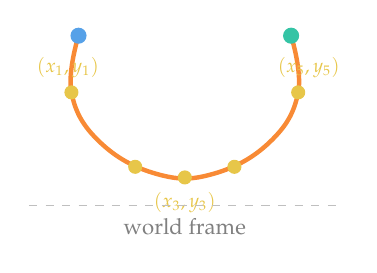
\begin{tikzpicture}[scale=0.9]
    \draw[RodOrange, line width=1.6pt]
        plot[smooth, tension=0.7] coordinates
        {(-1.5,1.0) (-1.6,0.2) (-1.2,-0.5) (-0.4,-0.95) (0.4,-0.95) (1.2,-0.5) (1.6,0.2) (1.5,1.0)};
    \filldraw[ArmBlue]   (-1.5,1.0)  circle (3pt);
    \filldraw[Armgreen]   (1.5,1.0)   circle (3pt);
    \foreach \p in {(-1.6,0.2),(-0.7,-0.85),(0,-1.0),(0.7,-0.85),(1.6,0.2)} {
        \filldraw[SampleYellow] \p circle (2.6pt);
    }
    \node[SampleYellow, font=\scriptsize] at (-1.65,0.55) {$(x_1,y_1)$};
    \node[SampleYellow, font=\scriptsize] at (0.0,-1.35) {$(x_3,y_3)$};
    \node[SampleYellow, font=\scriptsize] at (1.75,0.55) {$(x_5,y_5)$};
    \draw[gray!50, dashed] (-2.2,-1.4) -- (2.2,-1.4);
    \node[font=\footnotesize, gray] at (0,-1.7) {world frame};
\end{tikzpicture}
\caption{\textbf{Point coordinates.}\\ $\mathbf{s} = [\,x_i,y_i\,]_{i=1}^{5}$. Each entry is a
position in the world frame. If the object moves rigidly, changing position and
orientation without deforming, every entry of $\mathbf{s}$ changes, so this representation
registers rigid motion as a shape change.}
\label{fig:rep-points}
\end{subfigure}\hfill
\begin{subfigure}[t]{0.32\linewidth}
\centering
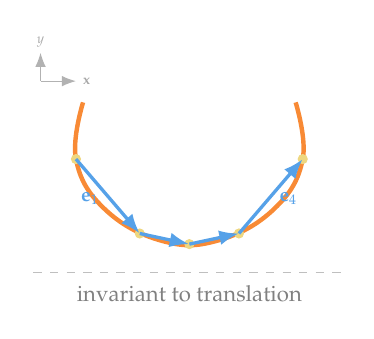
\begin{tikzpicture}[scale=0.9]
    \draw[RodOrange, line width=1.6pt]
        plot[smooth, tension=0.7] coordinates
        {(-1.5,1.0) (-1.6,0.2) (-1.2,-0.5) (-0.4,-0.95) (0.4,-0.95) (1.2,-0.5) (1.6,0.2) (1.5,1.0)};
    \foreach \p in {(-1.6,0.2),(-0.7,-0.85),(0,-1.0),(0.7,-0.85),(1.6,0.2)} {
        \filldraw[SampleYellow!70] \p circle (1.8pt);
    }
    \draw[ArmBlue, -{Latex[length=2.5mm]}, line width=1.2pt] (-1.6,0.2) -- (-0.7,-0.85);
    \draw[ArmBlue, -{Latex[length=2.5mm]}, line width=1.2pt] (-0.7,-0.85) -- (0,-1.0);
    \draw[ArmBlue, -{Latex[length=2.5mm]}, line width=1.2pt] (0,-1.0) -- (0.7,-0.85);
    \draw[ArmBlue, -{Latex[length=2.5mm]}, line width=1.2pt] (0.7,-0.85) -- (1.6,0.2);
    \node[ArmBlue, font=\scriptsize] at (-1.4,-0.35) {$\mathbf{e}_1$};
    \node[ArmBlue, font=\scriptsize] at (1.4,-0.35) {$\mathbf{e}_4$};
    \draw[gray!60, -{Latex[length=1.8mm]}] (-2.1,1.3) -- (-1.6,1.3);
    \draw[gray!60, -{Latex[length=1.8mm]}] (-2.1,1.3) -- (-2.1,1.7);
    \node[font=\tiny, gray!70] at (-1.45,1.3) {$\mathbf{x}$};
    \node[font=\tiny, gray!70] at (-2.1,1.85) {$y$};
    \draw[gray!50, dashed] (-2.2,-1.4) -- (2.2,-1.4);
    \node[font=\footnotesize, gray] at (0,-1.7) {invariant to translation};
\end{tikzpicture}
\caption{\textbf{Edge vectors.}\\ $\mathbf{e}_i = \mathbf{p}_{i+1}-\mathbf{p}_i$. A rigid translation
leaves the edge vectors unchanged: the rod could be carried five metres to the right
and $\mathbf{s}$ would be identical. A rigid \emph{rotation}, however, does change $\mathbf{s}$, because
every edge vector rotates with the rod. Edge vectors are therefore invariant to
translation but not to rotation.}
\label{fig:rep-edges}
\end{subfigure}\hfill
\begin{subfigure}[t]{0.32\linewidth}
\centering
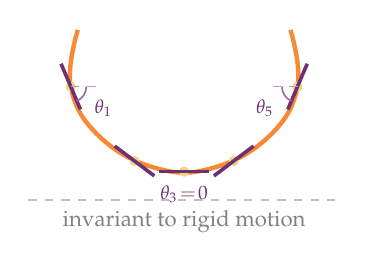
\begin{tikzpicture}[scale=0.9]
    \draw[RodOrange, line width=1.6pt]
        plot[smooth, tension=0.7] coordinates
        {(-1.5,1.0) (-1.6,0.2) (-1.2,-0.5) (-0.4,-0.95) (0.4,-0.95) (1.2,-0.5) (1.6,0.2) (1.5,1.0)};
    \foreach \p in {(-1.6,0.2),(-0.7,-0.85),(0,-1.0),(0.7,-0.85),(1.6,0.2)} {
        \filldraw[SampleYellow!70] \p circle (1.8pt);
    }
    \draw[Cat3Purple, line width=1.3pt]
        ($(-1.6,0.2)+(-67+180:0.35)$) -- ($(-1.6,0.2)+(-67:0.35)$);
    \draw[Cat3Purple!50, line width=0.5pt, dashed] (-1.6,0.2) -- ++(0:0.4);
    \draw[Cat3Purple!70, line width=0.6pt]
        (-1.6,0.2) ++(0:0.22) arc (0:-67:0.22);
    \node[Cat3Purple, font=\scriptsize] at ($(-1.6,0.2)+(-33:0.55)$) {$\theta_1$};
    \draw[Cat3Purple, line width=1.3pt]
        ($(-0.7,-0.85)+(-37+180:0.35)$) -- ($(-0.7,-0.85)+(-37:0.35)$);
    \draw[Cat3Purple, line width=1.3pt]
        ($(0,-1.0)+(180:0.35)$) -- ($(0,-1.0)+(0:0.35)$);
    \node[Cat3Purple, font=\scriptsize] at (0,-1.32) {$\theta_3\!=\!0$};
    \draw[Cat3Purple, line width=1.3pt]
        ($(0.7,-0.85)+(37+180:0.35)$) -- ($(0.7,-0.85)+(37:0.35)$);
    \draw[Cat3Purple, line width=1.3pt]
        ($(1.6,0.2)+(67+180:0.35)$) -- ($(1.6,0.2)+(67:0.35)$);
    \draw[Cat3Purple!50, line width=0.5pt, dashed] (1.6,0.2) -- ++(180:0.4);
    \draw[Cat3Purple!70, line width=0.6pt]
        (1.6,0.2) ++(180:0.22) arc (180:180+67:0.22);
    \node[Cat3Purple, font=\scriptsize] at ($(1.6,0.2)+(180+33:0.55)$) {$\theta_5$};
    \draw[gray!50, dashed] (-2.2,-1.4) -- (2.2,-1.4);
    \node[font=\footnotesize, gray] at (0,-1.7) {invariant to rigid motion};
\end{tikzpicture}
\caption{\textbf{Curvature (turning angles).}\\ $\theta_i$ is the local tangent direction
sampled along the rod; the curvature feature is the difference between consecutive directions,
$\kappa_i = \theta_{i+1}-\theta_i$. Because both rigid translation and rigid rotation
leave these differences unchanged, $\mathbf{s}$ then represents only the rod's intrinsic shape,
not its position or orientation: it is invariant to rigid motion.}
\label{fig:rep-curv}
\end{subfigure}
\caption{Three ways to represent the same U-shape with a finite feature vector $\mathbf{s}$. Each choice
leads to different characteristics regarding invariance to rigid translations or rotations.}
\label{fig:representations}
\end{figure}

\subsection*{What changes from one representation to the next}

The three representations carry progressively less information about where the rod \textit{is}
with respect to the world frame, and progressively more about its \textit{intrinsic} shape:

\begin{itemize}
    \item \textbf{Point coordinates.} A pure translation of the rod by $0.20$ [m] shifts every
    $x_i$ by $0.20$, so the measured change in error is large. This is the representation used
    in our 2D rod example.
    \item \textbf{Edge vectors.} Each entry is $\mathbf{e}_i = \mathbf{p}_{i+1}-\mathbf{p}_i$. A pure
    translation now leaves $\mathbf{s}$ unchanged; a rigid rotation does not, because the edge
    vectors rotate with the rod.
    \item \textbf{Curvature (turning angles).} Each entry is the turning angle between
    consecutive edges, $\kappa_i = \theta_{i+1}-\theta_i$, where $\theta_i$ is the direction of
    edge $\mathbf{e}_i$; the $P$ sampled points give $P-1$ edge directions and $P-2$ turning angles.
    Both rigid translation and rigid rotation leave $\mathbf{s}$ unchanged; only an actual change in
    shape affects $\mathbf{s}$.
\end{itemize}

\subsection*{The U-shape test}

Consider a rod with a U-shape that moves rigidly, i.e., it is translated and rotated without
undergoing material deformation. Sampling the rod at five points to define $\mathbf{s}$ as point
coordinates makes the feature state change substantially, whereas using the sampled curvature
values as $\mathbf{s}$ leaves it unchanged. Figure~\ref{fig:u-shape-verdict} illustrates this.

\begin{figure}[h!]
\centering
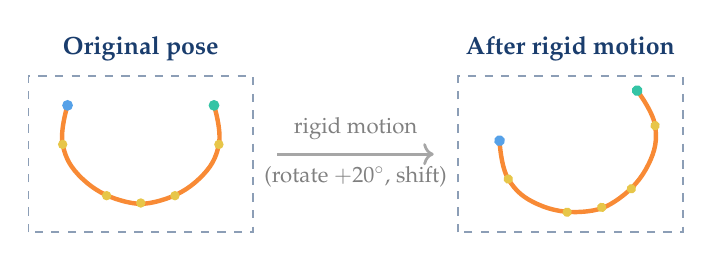
\begin{tikzpicture}[scale=0.62]
    \begin{scope}[xshift=-4.4cm]
        \draw[TitleBlue!50, line width=0.6pt, dashed] (-2.3,-1.6) rectangle (2.3,1.6);
        \node[anchor=south, font=\small\bfseries, TitleBlue] at (0,1.7) {Original pose};
        \draw[RodOrange, line width=1.6pt]
            plot[smooth, tension=0.7] coordinates
            {(-1.5,1.0) (-1.6,0.2) (-1.2,-0.5) (-0.4,-0.95) (0.4,-0.95) (1.2,-0.5) (1.6,0.2) (1.5,1.0)};
        \foreach \p in {(-1.6,0.2),(-0.7,-0.85),(0,-1.0),(0.7,-0.85),(1.6,0.2)} {
            \filldraw[SampleYellow] \p circle (2.4pt);
        }
        \filldraw[ArmBlue] (-1.5,1.0) circle (2.8pt);
        \filldraw[Armgreen] (1.5,1.0)  circle (2.8pt);
    \end{scope}
    \draw[->, gray!70, line width=1pt] (-1.6,0) -- (1.6,0);
    \node[gray, font=\footnotesize, anchor=south] at (0, 0.1) {rigid motion};
    \node[gray, font=\footnotesize, anchor=north] at (0,-0.05) {(rotate $+20^\circ$, shift)};
    \begin{scope}[xshift=4.4cm]
        \draw[TitleBlue!50, line width=0.6pt, dashed] (-2.3,-1.6) rectangle (2.3,1.6);
        \node[anchor=south, font=\small\bfseries, TitleBlue] at (0,1.7) {After rigid motion};
        \begin{scope}[xshift=0.3cm, yshift=-0.15cm, rotate=20]
            \draw[RodOrange, line width=1.6pt]
                plot[smooth, tension=0.7] coordinates
                {(-1.5,1.0) (-1.6,0.2) (-1.2,-0.5) (-0.4,-0.95) (0.4,-0.95) (1.2,-0.5) (1.6,0.2) (1.5,1.0)};
            \foreach \p in {(-1.6,0.2),(-0.7,-0.85),(0,-1.0),(0.7,-0.85),(1.6,0.2)} {
                \filldraw[SampleYellow] \p circle (2.4pt);
            }
            \filldraw[ArmBlue] (-1.5,1.0) circle (2.8pt);
            \filldraw[Armgreen] (1.5,1.0)  circle (2.8pt);
        \end{scope}
    \end{scope}
\end{tikzpicture}

\vspace{0.4em}
\renewcommand{\arraystretch}{1.35}
\begin{tabular}{@{} l c c c @{}}
\toprule
\textbf{Representation} & \textbf{Before} & \textbf{After} & $\bm{\|\Delta\mathbf{s}\|}$ \\
\midrule
Sample 1, point coords $(x_1,y_1)$
& $(-1.60,\;0.20)$
& $(-1.21,\;-0.42)$
& \multirow{2}{*}{\textcolor{Cat1Red}{\textbf{large}}} \\
Sample 3, point coords $(x_3,y_3)$
& $(\phantom{-}0.00,\;-1.00)$
& $(\phantom{-}0.64,\;-0.94)$
& \\
\midrule
Curvature $\kappa_i=\theta_{i+1}-\theta_i$, deg
& $(30,\;37,\;37,\;30)$
& $(30,\;37,\;37,\;30)$
& \textcolor{TargetGreen!50!black}{\textbf{0}} \\
\bottomrule
\end{tabular}
\caption{The same physical U-shape, before and after a rigid motion (translation and
rotation). Point-coordinate features change substantially; curvature features are
identical. Using point coordinates reflects a change in the state;  using curvature values does not.}
\label{fig:u-shape-verdict}
\end{figure}

No choice of $\mathbf{s}$ is universally correct; it depends on the objective. For example, use point
coordinates when the position of the rod matters, or use a rigid-motion-invariant
representation when only the shape matters. The choice of $\mathbf{s}$ also affects the Jacobian:
a gripper motion that produces $\dot{\mathbf{s}} \neq 0$ under one representation may produce
$\dot{\mathbf{s}} = 0$ under another. This relates directly to the observability discussed in
\S\ref{sec:taxonomy}.

Finally, representations can be combined. For instance, $\mathbf{s}$ may stack both point
coordinates and curvatures,
\[
    s=[\,x_1,y_1,\dots,x_P,y_P,\;\; \theta_{2}-\theta_1,\dots,\theta_{P}-\theta_{P-1}\,]^{\top}.
\]

\begin{labexercise}[Exercise~2]
Implement the three feature types (point coordinates, edge vectors, and curvature) as
functions of the rod's sampled points. Apply a rigid transformation to a U-shape, first a pure
translation and then a translation combined with a rotation, and for each feature map
compute the change $\|\Delta\mathbf{s}\|$ it induces. Confirm the results are coherent with the analysis from
Figure~\ref{fig:u-shape-verdict}.
(See \texttt{code/ex2\_representation.py}.)
\end{labexercise}

% ===========================================================
\section{Offline Jacobian estimation and its conditioning}
\label{sec:jacobian}

\subsection{The local linear map}
The controller's goal is to bring $\mathbf{s}$ to $\mathbf{s}^{*}$. Without a model of the rod, we
approximate how changes in robot configuration generate changes in feature space $\mathbf{s}$ through the local map $\mathbf{J}: \dot{\mathbf{r}}\mapsto \dot{\mathbf{s}}$, where $\mathbf{J}$ is the \emph{interaction
Jacobian} $\mathbf{J}(\mathbf{r})\in\mathbb{R}^{n\times m}$ (note that in our rod example $n=10$, $m=6$):
\begin{tcolorbox}[mathbox]
\begin{equation}
    \dot s \;=\; J(r)\,\dot r .
    \label{eq:fwd}
\end{equation}
\end{tcolorbox}
\noindent The mechanics that set $\mathbf{J}$ are unknown to the controller, so $\mathbf{J}$ cannot be
written down from a model: it must be estimated from data. \textbf{From now on $\mathbf{J}$ denotes
the \emph{true} interaction Jacobian, which the controller cannot observe, and $\hat{\mathbf{J}}$ its
estimate.}

\begin{intuition}[What a Jacobian is]
A Jacobian is the matrix counterpart of the \emph{slope} of a scalar function. For a scalar
$f(x)$, the slope $\mathrm{d}f/\mathrm{d}x$ describes how the output changes when the input
changes by a small amount. For a vector-valued $f$, the slope becomes a matrix whose entry
$J_{ij}$ describes how output $i$ changes when input $j$ changes. Here $J_{ij}$ answers the
following question: \emph{if gripper DoF $j$ of $\mathbf{r}$ moves by a small amount, say $0.01$~m,
by how much does sampled coordinate $i$ of $\mathbf{s}$ shift?} Column $j$ is therefore the shape
change, in feature space $\mathbf{s}$, produced by actuating DoF $j$ alone.
Figure~\ref{fig:jacobian} shows $\mathbf{J}$ as a heat-map of these columns.
\end{intuition}

\begin{figure}[h!]
    \centering
    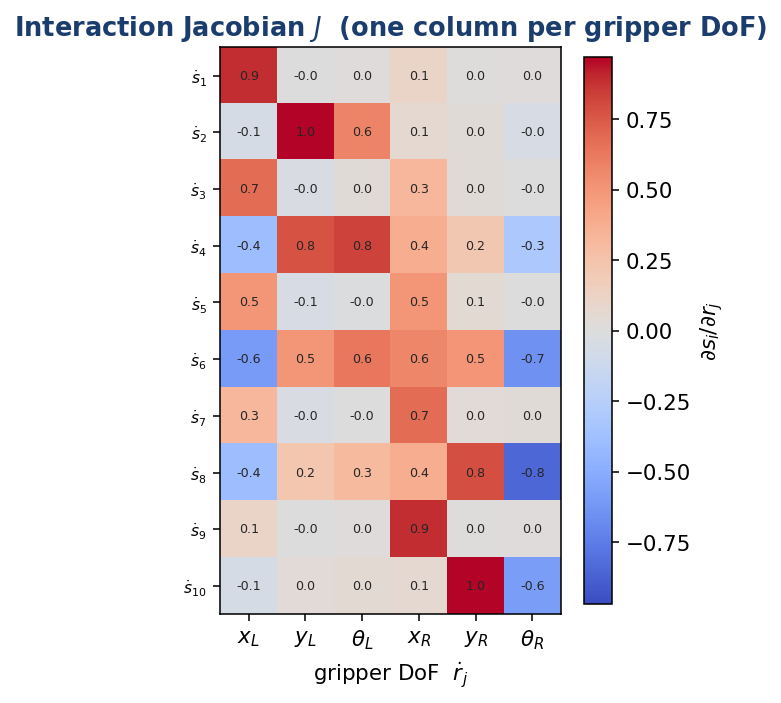
\includegraphics[width=0.62\linewidth]{figs/fig_jacobian.png}
    \caption{The interaction Jacobian as a heat-map. Each cell
    $(i,j)$ is $\partial s_i/\partial r_j$, that is, the influence of gripper DoF $j$ on feature
    $i$.}
    \label{fig:jacobian}
\end{figure}

\subsection{Offline estimation: regression from exploration data}
\label{sec:offline}

Before any closed-loop control begins, the controller commands a sequence of small
exploration motions and records the rod's response. We move each gripper DoF
independently at four amplitudes, giving $24$ measured pairs in total. Each pair is
$(\Delta\mathbf{r}_k,\,\Delta\mathbf{s}_k)$ with
\[
    \Delta r_k = r_k - r_0, \qquad \Delta s_k = s_k - s_0.
\]
Stacking these pairs column-wise gives the data matrices
\[
    \Delta R = [\Delta r_1, \dots, \Delta r_{24}] \in \mathbb{R}^{6 \times 24},
    \qquad
    \Delta S = [\Delta s_1, \dots, \Delta s_{24}] \in \mathbb{R}^{10 \times 24}.
\]
The initial estimate is the linear map that best explains $\Delta\mathbf{S} \approx \hat{\mathbf{J}}\,\Delta\mathbf{R}$
in a least-squares sense:
\begin{tcolorbox}[mathbox]
\begin{equation}
    \hat J^{(0)} \;=\; \arg\min_{\hat J}\, \|\Delta S - \hat J\,\Delta R\|_F^2
    \;=\; \Delta S\,\Delta R^{+},
    \label{eq:regression}
\end{equation}
\end{tcolorbox}
where $\Delta\mathbf{R}^{+} = \Delta\mathbf{R}^{\top}(\Delta\mathbf{R}\,\Delta\mathbf{R}^{\top})^{-1}$ is the right
Moore--Penrose pseudo-inverse of the wide exploration matrix $\Delta\mathbf{R}$ ($6\times 24$),
well defined as long as the exploration motions span all six DoF, which we guarantee by
actuating each DoF separately. The result is a $10\times 6$ matrix like the one in
Figure~\ref{fig:jacobian}, with one column per gripper DoF.

\begin{intuition}[Why this regression works]
Each exploration motion is one measurement: we apply a step $\Delta\mathbf{r}_k$ and record the
response $\Delta\mathbf{s}_k$. If the rod were exactly linear we would have
$\Delta\mathbf{s}_k = \mathbf{J}\Delta\mathbf{r}_k$ for one common $\mathbf{J}$ at every step. The rod is only
approximately linear over the exploration amplitudes, so the $24$ equations cannot all hold
exactly; we ask instead for the single $\hat{\mathbf{J}}$ that minimises the total squared
mismatch. Equation~\eqref{eq:regression} is the closed-form solution to that
least-squares problem.
\end{intuition}

\subsection{Span, rank, and conditioning}

For control we will invert $\hat{\mathbf{J}}$, so it must have full column rank and be well
conditioned. We characterise this through the span, rank, and singular values of the
Jacobian (read off the estimate $\hat{\mathbf{J}}^{(0)}$ in the lab), in the sense made precise by
the following definitions.

\begin{intuition}[\emph{Span}: which shape changes the grippers can reach]
The column span of $\mathbf{J}$ is the set of all $\dot{\mathbf{s}}$ that some choice of $\dot{\mathbf{r}}$ can
produce. Each column is the shape change from perturbing one gripper DoF; together the
six columns span at most a $6$-dimensional subspace of the $10$-dimensional shape
space. Shape changes inside the span can be commanded; those outside it cannot. Control
towards the target requires the column span of $\mathbf{J}$ to contain the deformation direction
the controller needs, i.e.\ the direction proportional to $\mathbf{s}^{*}-\mathbf{s}$.
\end{intuition}

\begin{intuition}[\emph{Rank}: the number of genuinely independent input directions]
The rank of $\mathbf{J}$ is the dimension of its column span. A $10\times 6$ Jacobian has rank at
most $6$; full column rank ($\mathrm{rank}(\mathbf{J})=6$) means each gripper DoF contributes a
shape change the others cannot reproduce. When the rank drops, there exist actions
$\dot{\mathbf{r}}\neq 0$ with $\dot{\mathbf{s}} = \mathbf{J}\dot{\mathbf{r}} = 0$: the grippers move, but the measured shape does
not.
\end{intuition}

A finer analysis comes from the singular value decomposition (SVD):
\begin{tcolorbox}[mathbox]
\begin{equation}
    J \;=\; U\,\Sigma\,V^{\top},\qquad
    \Sigma = \mathrm{diag}(\sigma_1,\dots,\sigma_6),\qquad
    \sigma_1 \geq \dots \geq \sigma_6 \geq 0.
\end{equation}
\end{tcolorbox}

\begin{intuition}[\emph{Singular values} $\sigma_i$: the gains of independent channels]
The SVD reorganises $\mathbf{J}$ into six independent channels. Each maps a particular combination
of gripper DoF (a column of $\mathbf{V}$) to a particular shape change (a column of $\mathbf{U}$), with
$\sigma_i$ as the scalar gain on that channel.

\smallskip
\noindent\textit{Scalar example.} With a single input and a single output (a $1\times 1$
Jacobian), say $J=2.5$, the only singular value is $\sigma_1=2.5$: an input $\dot r=0.01$
gives an output $0.025$. To invert, $J^{+}=1/\sigma_1=0.4$. If instead $\sigma_1=0.001$,
producing the same output needs an input of $25$, an amplification by a factor of $1000$.
At $\sigma_1=0$ the output is unreachable and the inverse does not exist. The matrix case
behaves the same
way along each channel: every $\sigma_i$ must be bounded away from zero for $\mathbf{J}^{+}$ to be
well conditioned.
\end{intuition}

The singular values yield two summary quantities:
\begin{tcolorbox}[mathbox]
\begin{equation}
    w \;=\; \sqrt{\det(J^{\top}J)} \;=\; \prod_i \sigma_i,
    \qquad
    \kappa \;=\; \sigma_{\max}/\sigma_{\min}.
\end{equation}
\end{tcolorbox}

\begin{intuition}[\emph{Manipulability} $w$ and \emph{condition number} $\kappa$]
$w$ is the product of all singular values, equal to the volume of the ellipsoid of shape
changes reachable by a small all-DoF perturbation. If any $\sigma_i\to 0$ the ellipsoid
collapses and $w\to 0$. Here $w$ measures the controller's overall capacity to actuate $\mathbf{s}$
in independent directions: \textbf{larger $w$ is better, and $w=0$ means at least one
direction of $\mathbf{s}$ can no longer be actuated.}

\smallskip
\noindent $\kappa$ is the ratio of the easiest to the hardest direction to actuate
(largest over smallest $\sigma_i$). $\kappa=1$ means every direction responds equally;
$\kappa\to\infty$ as $\sigma_{\min}\to 0$. \textbf{Smaller $\kappa$ is better; a very
large $\kappa$ signals a direction that produces almost no change in $\mathbf{s}$.}
\S\ref{sec:taxonomy} tracks $\sigma_{\min}$, $w$, and $\kappa$ together as they collapse
near a singularity.
\end{intuition}

\begin{labexercise}[Exercise~3]
Estimate the interaction Jacobian $\hat{\mathbf{J}}^{(0)}$ at the nominal EE pose by offline
regression: explore each DoF, gather the input/output changes $\Delta\mathbf{R},\Delta\mathbf{S}$, and fit
$\hat{\mathbf{J}}^{(0)}=\Delta\mathbf{S}\,\Delta\mathbf{R}^{+}$. Read its rank, manipulability $w$, and condition
number $\kappa$ from the SVD.
(See \texttt{code/ex3\_offline\_jacobian.py}.)
\end{labexercise}

% ===========================================================
\section{Closing the loop and the online update}
\label{sec:estimation}

With a well-conditioned estimate $\hat{\mathbf{J}}$ in hand (\S\ref{sec:jacobian}), the controller
inverts it to drive the shape, and refreshes it online as the rod deforms away from where
it was measured.

\subsection{Closing the loop}

The controller closes the loop by inverting the estimate. A clean inverse $\hat{\mathbf{J}}^{-1}$
exists only for a square, full-rank matrix. Here $\hat{\mathbf{J}}\in\mathbb{R}^{n\times m}$ with
$n=10>m=6$: it is rectangular (more shape features than actuation DoF) and therefore not
invertible in the usual sense. We use the Moore--Penrose pseudo-inverse $\hat{\mathbf{J}}^{+}$:
\begin{tcolorbox}[mathbox]
\begin{equation}
    \Delta r \;=\; \alpha\, \hat J^{+}(s^{*}-s),
    \qquad \hat J^{+} = (\hat J^{\top}\hat J)^{-1}\hat J^{\top}.
    \label{eq:ctrl}
\end{equation}
\end{tcolorbox}

\begin{intuition}[The \emph{pseudo-inverse} $\hat{\mathbf{J}}^{+}$]
For a tall, full-column-rank $\hat{\mathbf{J}}$, the Moore--Penrose pseudo-inverse
$\hat{\mathbf{J}}^{+}=(\hat{\mathbf{J}}^{\top}\hat{\mathbf{J}})^{-1}\hat{\mathbf{J}}^{\top}$ is the best linear substitute for an inverse: given an
error $\mathbf{e}=\mathbf{s}^{*}-\mathbf{s}$, the step $\hat{\mathbf{J}}^{+}\mathbf{e}$ is the $\Delta\mathbf{r}$ whose predicted shape change
$\hat{\mathbf{J}}\Delta\mathbf{r}$ is closest to $\mathbf{e}$ in the least-squares sense. In SVD coordinates $\hat{\mathbf{J}}^{+}$ acts
on channel $i$ with gain $1/\sigma_i$. This is why a small $\sigma_i$ in $\hat{\mathbf{J}}$ becomes a
large gain in $\hat{\mathbf{J}}^{+}$: the controller commands large gripper motions precisely along the
directions in which the rod responds least.
\end{intuition}

\begin{figure}[h!]
    \centering
    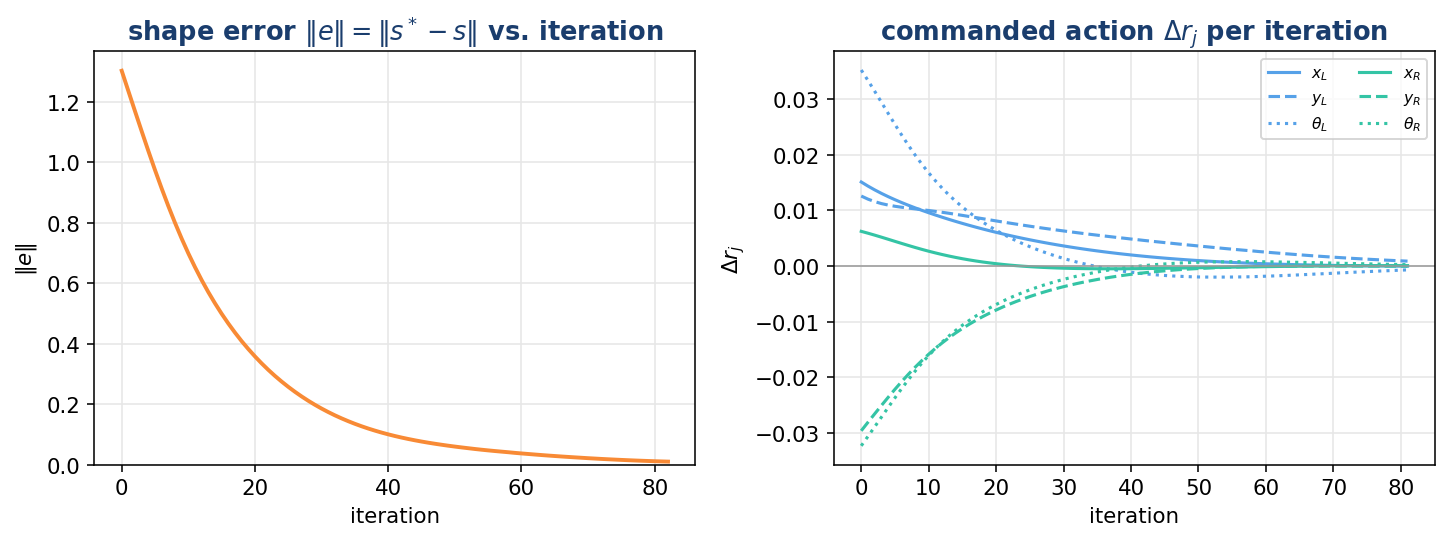
\includegraphics[width=0.92\linewidth]{figs/fig_control.png}
    \caption{The closed loop in operation, with a small gain $\alpha=0.05$.
    \emph{Left:} the shape error $\|\mathbf{e}\|$ falls smoothly and steadily towards zero as
    the pseudo-inverse step $\Delta\mathbf{r}=\alpha \hat{\mathbf{J}}^{+}\mathbf{e}$ is applied and the rod is
    re-measured. \emph{Right:} the commanded action $\Delta\mathbf{r}_j$ at each iteration,
    which shrinks to zero as the error vanishes.}
    \label{fig:closed-loop}
\end{figure}

\subsection{Online update: the Broyden rule}
\label{sec:online}

The offline estimate is local: it is accurate near the initial configuration $\mathbf{r}_0$ where
it was measured, but as the control loop runs and the rod deforms, the true $\mathbf{J}(\mathbf{r})$
changes and $\hat{\mathbf{J}}^{(0)}$ loses accuracy. To keep $\hat{\mathbf{J}}$ current, the controller updates
it at every iteration using the data the loop already produces.

\smallskip
At iteration $k$ the robot commanded a step $\Delta\mathbf{r}$ and observed a shape change
$\Delta\mathbf{s}$. If $\hat{\mathbf{J}}$ were exact we would have $\Delta\mathbf{s} = \hat{\mathbf{J}}\,\Delta\mathbf{r}$; in general
there is a residual $\Delta\mathbf{s} - \hat{\mathbf{J}}\,\Delta\mathbf{r}\neq 0$ quantifying what the estimate
failed to predict. The \emph{Broyden update} corrects $\hat{\mathbf{J}}$ to absorb that residual:
\begin{tcolorbox}[mathbox]
\begin{equation}
    \hat J^{(k+1)} \;=\; \hat J^{(k)} \;+\; \frac{\big(\Delta s - \hat J^{(k)}\,\Delta r\big)\,\Delta r^{\top}}{\Delta r^{\top}\,\Delta r},
    \label{eq:broyden}
\end{equation}
\end{tcolorbox}
with $\Delta\mathbf{r} = \mathbf{r}^{(k+1)} - \mathbf{r}^{(k)}$ and $\Delta\mathbf{s} = \mathbf{s}^{(k+1)} - \mathbf{s}^{(k)}$.

\begin{intuition}[What Broyden is doing]
The numerator is the prediction error: what the rod actually did, minus what $\hat{\mathbf{J}}$
predicted. The outer product with $\Delta\mathbf{r}^{\top}$ projects that error back along the
direction just moved, and the denominator $\|\Delta\mathbf{r}\|^{2}$ normalises by the size of the
step. Adding this rank-one correction yields the updated $\hat{\mathbf{J}}^{(k+1)}$ used at the next
step.

\smallskip
\noindent The update is the multivariable generalisation of a secant slope: with no
analytical model of the rod, we refine the estimate using the data measured during
control. The sensitive term is the denominator. When $\|\Delta\mathbf{r}\|$ is small but
$\|\Delta\mathbf{s}\|$ is large, the factor $1/\|\Delta\mathbf{r}\|^2$ makes the correction arbitrarily
large. \S\ref{sec:taxonomy} (Category~3) returns to this: at a mechanical instability such
as buckling, a tiny $\Delta\mathbf{r}$ produces a large $\Delta\mathbf{s}$, so Eq.~\eqref{eq:broyden}
injects a large spurious correction into $\hat{\mathbf{J}}$, and the next pseudo-inverse commands no
longer reflect the rod's true response.
\end{intuition}

\subsection{Three conditions for good closed-loop control}

With $\hat{\mathbf{J}}$ in the loop, three conditions must hold at once. Each one also governs the
offline exploration and the online update, so any of them can fail at the start of the task
or appear partway through it:

\begin{enumerate}
    \item \textbf{Controllability / reachability.} The columns of the true $\mathbf{J}$ span the
    shape changes needed to reach $\mathbf{s}^{*}$, and the estimate $\hat{\mathbf{J}}$ has not collapsed its
    own column span, so the inverse map $\hat{\mathbf{J}}^{+}$ remains well defined.
    \item \textbf{Observability.} The chosen features $\mathbf{s}$ register the rod's physical
    evolution, so the measured $\Delta\mathbf{s}$ feeding Eq.~\eqref{eq:broyden} is informative.
    \item \textbf{Linearity.} The model $\dot{\mathbf{s}} = \mathbf{J}\dot{\mathbf{r}}$ remains a good local
    approximation, and $\Delta\mathbf{s}$ comes from that smooth regime rather than from a
    discontinuous response.
\end{enumerate}

\noindent Each of the next three categories corresponds to one of these conditions failing.

\begin{labexercise}[Exercise~4]
Starting from the offline estimate $\hat{\mathbf{J}}^{(0)}$ of Exercise~3, add the Broyden update of
Eq.~\eqref{eq:broyden} and complete the closed control loop that drives $\mathbf{s}$ to the target.
With the Broyden update on the loop converges quickly; with a fixed estimate it converges
much more slowly.
(See \texttt{code/ex4\_control\_loop.py}.)
\end{labexercise}

\newpage
% ===========================================================
\section{Three ways the loop fails}
\label{sec:taxonomy}

% --- CATEGORY 1 ---
\begin{physbox}
\textbf{Analytical side.} The grippers move, but the resulting shape change is negligible.
Some direction of gripper motion leaves the physical system essentially unchanged, so the columns of $\mathbf{J}$
along that direction shrink (DoF $\dot{\mathbf{r}}_j$ loses influence on the rod):
$\sigma_{\min}(\mathbf{J})\to 0$, $w\to 0$, $\kappa\to\infty$. When the controller asks $\mathbf{J}^{+}$ to
correct an error along that direction, the gain $1/\sigma_{\min}$ grows without bound: the
commanded gripper step becomes large while the shape changes very little.

\medskip
\noindent\textbf{Broyden update.} The estimate receives $\Delta\mathbf{r} \neq 0$ but
$\Delta\mathbf{s} \approx 0$. The residual reduces to $-\hat{\mathbf{J}}\,\Delta\mathbf{r}$, so the update shrinks
$\hat{\mathbf{J}}$'s column along $\Delta\mathbf{r}$. After a few iterations $\hat{\mathbf{J}}$ also reports that
direction as inactive, which is precisely the direction the controller still needs in
order to move the shape.

\medskip
\noindent\textbf{Where it arises.}
\begin{itemize}
    \item \emph{Taut state.} The rod is pulled straight; outward gripper motion
    produces no $\dot{\mathbf{s}}$, only tension. Figure~\ref{fig:taut} increases the separation
    through this regime and shows $\sigma_{\min}(\mathbf{J})$ collapsing.
    \item \emph{Slack state.} The grippers are closer than the rod's resting length;
    gripper motion is taken up by the slack rather than transmitted through the rod.
    \item \emph{Rigid-body and symmetry redundancies.} Several gripper motions
    produce the same $\dot{\mathbf{s}}$, so $\mathbf{J}$ is genuinely rank-deficient on its input side.
\end{itemize}
\end{physbox}

\begin{figure}[h!]
    \centering
    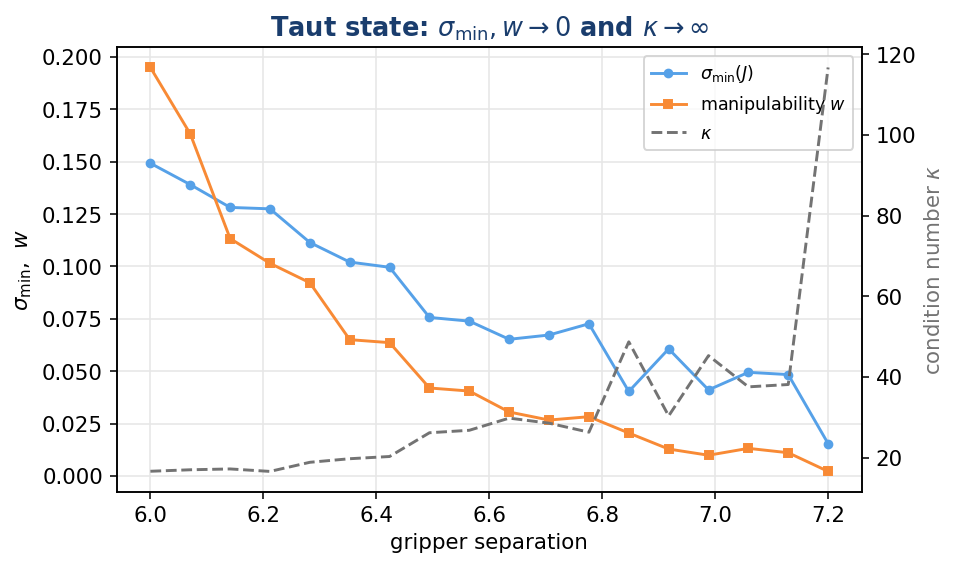
\includegraphics[width=0.78\linewidth]{figs/fig_taut.png}
    \caption{Taut state (Category 1). As the gripper separation grows, the rod is pulled into
    tension: $\sigma_{\min}(\mathbf{J})$ and the manipulability $w$ collapse while the condition
    number $\kappa$ rises from about $17$ to $117$. The pseudo-inverse would amplify
    commands as $1/\sigma_{\min}$ to keep the shape moving.}
    \label{fig:taut}
\end{figure}

\newpage

% --- CATEGORY 2 ---
\begin{obsbox}
\textbf{Analytical side.} The rod \emph{is} deforming in response to gripper motion, but
the chosen features $\mathbf{s}$ are insensitive to that particular deformation. Now the rows of
$\mathbf{J}$, not the columns, are the problem: $\dot{\mathbf{s}} \approx 0$ because of the features, so the
controller receives an uninformative $\Delta\mathbf{s}\approx 0$ even though the rod actually
moved.

\medskip
\noindent The link to \S\ref{sec:representation} is direct: this is what happens when the
representation is too coarse, too symmetric, or too invariant to register the change.

\medskip
\noindent\textbf{Broyden update.} The numerical signature is the same as Category~1 (a
non-zero $\Delta\mathbf{r}$ paired with $\Delta\mathbf{s}\approx 0$), but the cause is the feature map
rather than the physics. The relevant rows of $\hat{\mathbf{J}}$ decay toward zero, so the
controller stops attributing any feature response to those gripper directions.

\medskip
\noindent\textbf{Where it arises.}
\begin{itemize}
    \item \emph{Sub-parametrised features.} Twisting a smooth, untextured rod about its
    axis: the material twists but the sampled centreline does not move.
    \item \emph{Symmetric features.} Move one gripper up by the same amount the
    other moves down. The rod clearly deforms, but a scalar feature such as the midpoint
    height stays at zero. Figure~\ref{fig:observability} shows this case.
    \item \emph{Self-occlusion.} A folded garment hides part of itself; rows of $\mathbf{s}$ vanish
    mid-task.
\end{itemize}
\end{obsbox}

\begin{figure}[h!]
    \centering
    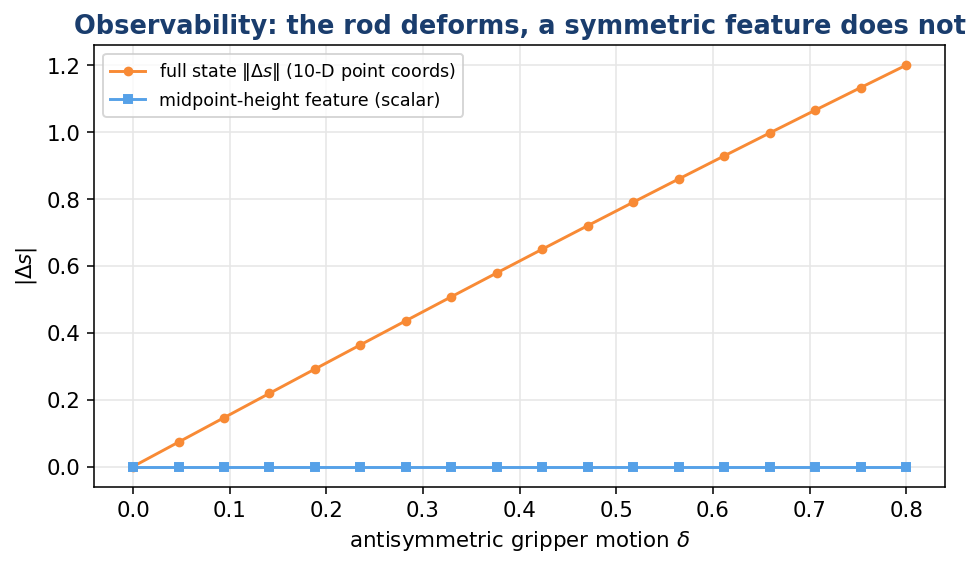
\includegraphics[width=0.78\linewidth]{figs/fig_observability.png}
    \caption{Observability (Category 2). An antisymmetric vertical motion (one gripper up,
    the other down) clearly deforms the rod, so the full $10$-D point-coordinate state
    grows steadily; yet a single symmetric scalar feature (the midpoint height)
    stays at zero and does not register the deformation.}
    \label{fig:observability}
\end{figure}

\newpage

% --- CATEGORY 3 ---
\begin{dynbox}
\textbf{Analytical side.} Categories~1 and~2 were both rank deficiencies of $\mathbf{J}$. This one
is qualitatively different: the linear model itself ceases to hold. A small input
$\dot{\mathbf{r}}$ produces a large, near-discontinuous $\dot{\mathbf{s}}$, and no finite matrix $\mathbf{J}$ can
describe that relationship.

\medskip
\noindent The mechanical reason is that the rod stores internal elastic energy as it
strains, and at certain configurations the Hessian of the elastic potential loses
positive definiteness:
\begin{tcolorbox}[mathbox, width=0.85\linewidth, center]
\begin{equation}
    \det\!\big(H_{\mathrm{energy}}\big) \;=\; 0
    \qquad\Longleftrightarrow\qquad
    \lambda_{\min}(H_{\mathrm{energy}}) \;\to\; 0.
    \label{eq:bif}
\end{equation}
\end{tcolorbox}
\noindent The current equilibrium ceases to be stable; the rod releases the stored elastic
energy and settles into a different equilibrium shape on its own.

\medskip
\noindent\textbf{Broyden update.} During the snap the gripper moved very little
($\|\Delta\mathbf{r}\|$ small) while the shape changed by a large amount ($\|\Delta\mathbf{s}\|$ large). In
Eq.~\eqref{eq:broyden},
\[
    \hat J^{(k+1)} - \hat J^{(k)}
    \;=\;
    \frac{\overbrace{(\Delta s - \hat J^{(k)}\Delta r)}^{\text{very large}}\,\Delta r^{\top}}{\underbrace{\|\Delta r\|^2}_{\text{very small}}},
\]
so the numerator is dominated by the large $\Delta\mathbf{s}$ and the denominator is the square of
a tiny step. A single iteration injects a large spurious correction into $\hat{\mathbf{J}}$, and the
next pseudo-inverse $\hat{\mathbf{J}}^{+}$ produces commands unrelated to the rod's actual response.

\medskip
\noindent\textbf{Where it arises.}
\begin{itemize}
    \item \emph{Euler buckling.} Axial compression. The straight rod is stable
    until $\lambda_{\min}(\mathbf{H}_{\mathrm{energy}})$ crosses zero, then snaps sideways.
    \item \emph{Bi-stable snap-through.} A pre-curved shell pushed past an energy barrier
    snaps to a second equilibrium.
    \item \emph{Supercoiling.} Twisting a rubber cord steadily: torque rises linearly until
    the rod buckles into a helical writhe.
\end{itemize}
\end{dynbox}

\begin{intuition}[\emph{Energy Hessian} and \emph{positive definiteness}]
A rod at rest sits at a local minimum of its elastic potential energy $U(\mathbf{x})$, where $\mathbf{x}$ is
the rod's physical configuration. Near that minimum $\mathbf{U}$ looks like a bowl: every small
perturbation increases the stored energy, so the rod is pushed back to rest. The Hessian
$\mathbf{H}_{\mathrm{energy}} = \partial^{2}U/\partial \mathbf{x}^{2}$ describing this bowl has all positive
eigenvalues: it is positive definite, curving upward in every direction (a ball placed
inside returns to the bottom). When the smallest eigenvalue drops to zero, the bowl
flattens in one direction, like a trough. Past that point the eigenvalue is negative and
the bowl becomes a saddle: the equilibrium is unstable, and a small perturbation sends the
rod to a different shape far away. That is a buckling event, and there the linear model
$\dot{\mathbf{s}} = \mathbf{J}\dot{\mathbf{r}}$, which presumes a deep, stable bowl, no longer applies.
\end{intuition}

\begin{figure}[h!]
    \centering
    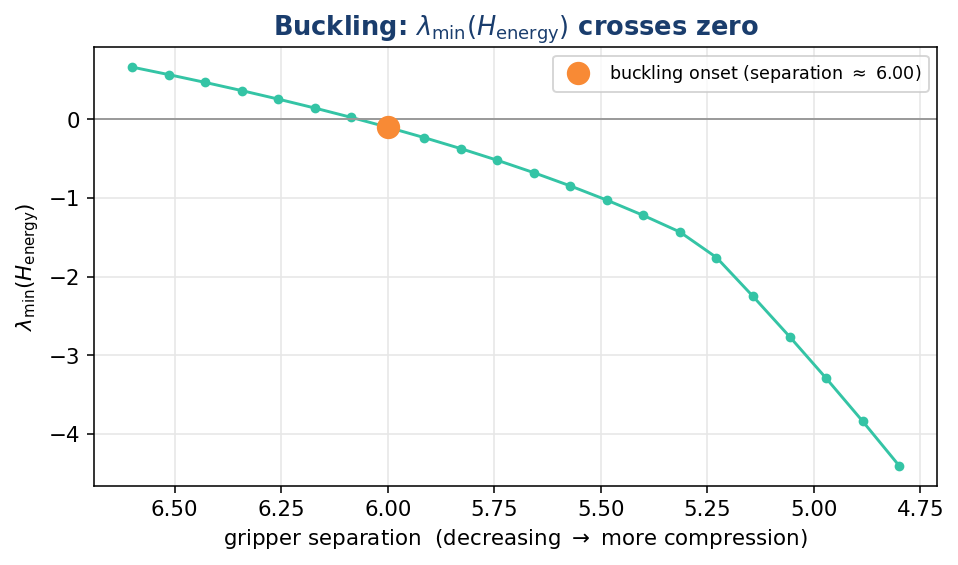
\includegraphics[width=0.78\linewidth]{figs/fig_buckling.png}
    \caption{Buckling (Category 3). As the gripper separation decreases the rod is axially
    compressed. The smallest eigenvalue of the straight-rod energy Hessian crosses zero
    (marked); below that separation the straight equilibrium is unstable and the rod snaps
    sideways.}
    \label{fig:buckling}
\end{figure}

\begin{labexercise}[Exercise~5]
Reproduce all three failure modes with the same rod and Jacobian tools: increase the
gripper separation and observe $\sigma_{\min}$, $w$, and $\kappa$ collapse in the taut
state (Figure~\ref{fig:taut}); apply an antisymmetric motion to expose a feature
insensitive to the deformation (Figure~\ref{fig:observability}); and compress the rod until
$\lambda_{\min}(\mathbf{H}_{\mathrm{energy}})$ crosses zero (Figure~\ref{fig:buckling}).
(See \texttt{code/ex5\_failure\_modes.py}.)
\end{labexercise}

\newpage
% ===========================================================
\section{Summary}
\label{sec:summary}

\begin{center}
\renewcommand{\arraystretch}{1.55}
\begin{tabular}{@{} p{3.4cm} p{2.8cm} p{4.4cm} p{4.0cm} @{}}
\toprule
\textbf{Category} & \textbf{What breaks} & \textbf{Analytical failure} & \textbf{Effect on $\hat{\mathbf{J}}$ (Broyden)} \\
\midrule
\textbf{1.} Controllability\newline (taut, slack, redundancy) & Columns of $\mathbf{J}$ & $\sigma_{\min}(\mathbf{J})\to 0$, $w\to 0$, $\kappa\to\infty$. $\mathbf{J}^{+}$ amplifies error by $1/\sigma_{\min}$. & $\Delta\mathbf{r}\neq 0$, $\Delta\mathbf{s}\approx 0$. Update shrinks $\hat{\mathbf{J}}$'s column toward zero. \\
\rowcolor{black!5}
\textbf{2.} Observability\newline (textureless or over-symmetric features) & Rows of $\mathbf{J}$ & Rank drop on the output side. $\dot{\mathbf{s}}\approx 0$ even though the rod moves; no shape-change signal, $\Delta\mathbf{s} \approx 0$. & Same signature as Category~1, with the feature map as the cause. The relevant rows of $\hat{\mathbf{J}}$ decay. \\
\textbf{3.} Mechanical instabilities\newline (buckling, snap-through, supercoiling) & The relation $\dot{\mathbf{s}} = \mathbf{J}\dot{\mathbf{r}}$ itself & $\det(\mathbf{H}_{\mathrm{energy}})=0$. A small $\dot{\mathbf{r}}$ produces a large, autonomous $\dot{\mathbf{s}}$; no finite $\mathbf{J}$ describes it. & $\|\Delta\mathbf{r}\|$ small, $\|\Delta\mathbf{s}\|$ large. $1/\|\Delta\mathbf{r}\|^2$ injects a large spurious correction into $\hat{\mathbf{J}}$ in one step. \\
\bottomrule
\end{tabular}
\end{center}

\vspace{1em}
\noindent A robust shape-control loop needs $\mathbf{J}$ well-conditioned (Category~1), features
that actually register the deformation (Category~2, with \S\ref{sec:representation} as the
broader context), and the linear model to remain valid (Category~3). Because $\hat{\mathbf{J}}$ is
updated online by Eq.~\eqref{eq:broyden}, each failure has two effects: the immediate
inversion is unreliable, and the estimate the next iteration relies on is degraded. The three
categories map exactly onto the three preconditions of \S\ref{sec:online}, and the lab of
\S\ref{sec:taxonomy} reproduces each one in isolation.

\end{document}
